% common part for every lection

\documentclass{beamer}

\usetheme{Warsaw}
\usefonttheme[onlylarge]{structurebold}
\setbeamerfont*{frametitle}{size=\normalsize,series=\bfseries}
\setbeamertemplate{navigation symbols}{}

\usepackage{pdfpages}
\usepackage{soul}
\usepackage{ucs}
\usepackage[utf8x]{inputenc}
\usepackage[TS1,T2A]{fontenc}
\usepackage[english,russian]{babel}
\usepackage{times}
\usepackage{listings}

\author[Author, Vlad Shakhov]{Влад 'mend0za' Шахов\\Linux \& Embedded Team Leader}

\institute[SaM Solutions]
{
  Linux \& Embedded Department
}

\date[Dec 2012]

\subject{Linux QA training}

\pgfdeclareimage[height=1.5cm]{sam-solutions-logo}{clipart/sam-solutions-elinux}

\logo{\pgfuseimage{sam-solutions-logo}}

\graphicspath{{./clipart/}}



\title[SaM Solutions. Linux QA Training]
{
  Занятие 2.\\
  Bourne Shell aka POSIX sh.
}

\begin{document}
\begin{frame}
  \titlepage
\end{frame}

\section{Введение в Shell}

\begin{frame}
  \frametitle{Что такое Unix shell?}
  
  \alert{Что такое Unix shell? (Назойливый повтор)}

  \begin{itemize}
    \item Обычная программа, запускающаяся после входа в систему
    \item Интерактивный командный интерпретатор
    \item Язык программирования
    \item Платформа интеграции (для утилит)
    \item Сотни разных реализаций (bash, ksh, zsh, tcsh, \ldots )
    \item Масса различных диалектов
  \end{itemize}

\end{frame}

\begin{frame}[fragile]
  \frametitle{Shell. Ключевые понятия - 1}
  \framesubtitle{Определения}

  \begin{itemize}
    \item \alert{Приглашение командной строки (CMD PROMPT)}: \pause 
      \begin{verbatim}
	$, #, user@host:~$
      \end{verbatim} \pause
    \item \alert{Команда}: \newline \verb+whoami; top; exit+ \pause
    \item \alert{Параметр}: \newline \verb+man bash; who am i+ \pause
    \item \alert{Ключ (1 символ)}: \newline \verb+ls -a; ls -al; ls -a -l /tmp/+ \pause
    \item \alert{Длинный ключ (GNU-style}: \newline \verb+ls --version+
  \end{itemize}
\end{frame}

\begin{frame}
  \frametitle{Shell. Ключевые понятия - 2}
  \framesubtitle{Картинка для закрепления}
    \hbox{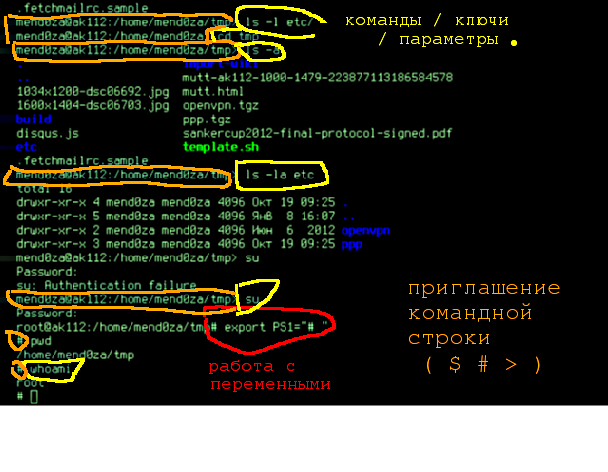
\includegraphics[height=7cm]{bash-input-screenshot}}
\end{frame}

\subsection{Интерактивная работа в Shell}

\begin{frame}
  \frametitle{Приёмы эффективной работы}

  \alert{\Large{Как в Shell работать быстро?}} 
  \pause

  \begin{enumerate}
    \item \Large{автодополнение путей и команд}
    \item \Large{история команд}
    \item \Large{редактирование командной строки}
  \end{enumerate}

\end{frame}

\begin{frame}[fragile]
  \frametitle{Приёмы эффективной работы}
  \framesubtitle{Автодополнение путей и команд - 1}

  \alert{\Large{Волшебная кнопка - TAB}} \newline
  \pause
  \begin{itemize}
    \item \Large{Имя команды} \pause \newline
      \small{Пример: \verb+mys[TAB]_co[TAB]+} \pause \newline
      \small{Результат: \verb+mysql_convert_table_format+} \newline
      \alert{8 vs 26} \pause
    \item \Large{Пути и имена файлов} \pause \newline
      \small{Пример: \verb+ls /u[TAB]lo[TAB]sh[TAB]/ca[TAB]+} \pause \newline
      \small{Результат: \verb+ls /usr/local/share/ca-certificates/+} \newline
      \alert{16 vs 36} \pause
    \item \Large{Параметры и ключи} \footnote{Только у BASH и ZSH (если настроены)} \pause \newline
      \small{Пример: \verb+apti[TAB]--a[TAB]sh[TAB]core[TAB][ENTER]+} \pause \newline
      \small{Результат: \verb+aptitude --assume-yes show coreutils+} \newline
      \alert{16 vs 37} \pause
  \end{itemize}
\end{frame}

\begin{frame}
  \frametitle{Приёмы эффективной работы}
  \framesubtitle{Автодополнение путей и команд - 2}
  
  \Large{\alert{Единственный вариант подстановки}: \newline TAB дополняет сразу} \pause

  \Large{\alert{Несколько вариантов подстановки?}} 

  \Large{Ещё больше волшебства - 2 кнопки TAB!} 

  \Large{\alert{2xTAB - список вариантов подстановки}}
\end{frame}

\begin{frame}[fragile]
  \frametitle{Приёмы эффективной работы}
  \framesubtitle{Автодополнение путей и команд - 3}
  
  \Huge{Примеры}

  \Large{
  \begin{itemize}
    \item apt[TAB][TAB]
    \item \verb+aptitude --[TAB][TAB]+\footnote{Только для BASH и ZSH}
    \item ls /[TAB][TAB] \footnote{Можно использовать вместо команды ``ls''}
  \end{itemize}
      }
\end{frame}
  

\begin{frame}
  \frametitle{Приёмы эффективной работы}
  \framesubtitle{История команд}

  \Large{\alert{Просмотр истории}}

  \begin{itemize}
    \item ``Up'' и ``Down'' - вперёд-назад \pause
    \item ``Ctrl+R'' - интерактивный поиск в истории \pause
    \item повторно ''Ctrl+R`` - искать дальше
  \end{itemize}
\end{frame}

\begin{frame}
  \frametitle{Приёмы эффективной работы}
  \framesubtitle{Редактирование командной строки}

  \Large{\alert{Emacs editing mode}} \footnote{Только KSH-совместимые: bash, zsh, pdksh, mksh, etc}

  \begin{itemize}
    \item ``Left'' и ``Right'' - вперёд-назад по текущей строке \pause
    \item ``Ctrl+a'' и ``Ctrl+e''  - перейти в начало и конец строки \pause
    \item ``Ctrl+u'' - удалить от курсора до начала строки \pause
    \item ``Ctrl+w'' - удалить слово (от курсора до разделителя, влево) 
  \end{itemize}
    
\end{frame}

\section{Выполнение команд и скриптов}

\subsection{Код возврата}

\begin{frame}[fragile]
  \frametitle{Условное выполнение команд}

  \Large{\alert{Код возврата (RETURN CODE)}}: \newline 
  \normalsize{результат выполнения у любой команды Shell}
  \newline

  Shell return code:
  \begin{itemize}
    \item 0 - выполнень успешно
    \item не 0 - ошибка
  \end{itemize}
  \pause

  Операции над кодом возврата:
  \begin{itemize}
    \item ``\verb+&&+'' - логическое И
    \item ``\verb+||+'' - логическое ИЛИ
  \end{itemize}
  \pause

  Примеры:
  \begin{itemize}
    \item \verb+ cat /proc/1/environ || echo fail +
    \item \verb+ find /usr/share/doc -name ``*.txt'' && echo ok+
  \end{itemize}

\end{frame}

\subsection{Скрипты}

\begin{frame}[fragile]
  \frametitle{Скрипты}
 
  \begin{block}<1->{Shell Script, определение}  

    Последовательность команд Shell.

    Разделитель: перевод строки, ``;''
  \end{block}

  \begin{block}<2->{shebang}
    \verb+#!something+ или чем мы запускаем скрипт. 
    
    По умолчанию : \verb+#!/bin/sh+
  
    Всегда первая строка скрипта.

    Фактически: \verb+/bin/sh scriptname+
  \end{block}

  \begin{block}<3->{Парадоксальные примеры}
    \verb+#!/bin/rm+

    \verb+#!/bin/awk -f+

    \verb+#!/bin/less+
  \end{block}

\end{frame}

\begin{frame}[fragile]
  \frametitle{Запуск скриптов}
  \begin{enumerate} 
    \item \verb+sh scriptname+
    \item \verb-chmod +x script- \newline \verb+./script+
    \item из каталогов в переменной PATH 
      \newline \verb+echo $PATH+
      \newline \verb+~/bin+ (если есть)
      \newline \verb+/usr/local/bin+
    \item в текущей копии shell\footnote{ Остальные способы - запускают новый shell}
      \newline \verb+. ./script+
      \newline \verb+source script+\footnote{ Несовместимо с POSIX. Происходит из ksh. Добавляет текущий каталог к списку путей}
  \end{enumerate}
\end{frame}

\section{Перенаправление ввода-вывода}
\begin{frame}
  \frametitle{Потоки ввода-вывода}
  
  Особенности архитектуры\footnote{См документацию языка программирования Си}:
  \begin{block}<1->{У каждой запущенной программы 3 потока I/O:}
    \begin{enumerate}
      \setcounter{enumi}{-1}
      \item ввода
      \item вывода
      \item ошибок
    \end{enumerate}

    Cвязаны с экраном и клавиатурой терминала. \pause \newline
  \end{block}

  \begin{block}<2->{Связаны с терминалом только по умолчанию}

    \alert{shell позволяет переопределить весь ввод и вывод программы}
  \end{block}

\end{frame}

\begin{frame}[fragile]
  \frametitle{Базовый cинтаксис перенаправления}
  \begin{itemize}    
    \item \alert{Ввод} ``<'' \newline
      \verb+ sort <.bash_history+ \pause
    \item \alert{Вывод} ``>'' \footnote{Файл затрёт новым содержанием, если он существовал ранее} \newline
      \verb+ find /usr/share/doc -name ``*.txt'' >txt-docs+    
    \item \alert{Вывод} ``1>'' \newline
      \verb+ find /usr/share/doc -name ``*.txt'' 1>txt-docs+ \pause
    \item \alert{Ошибки} ``2>''\newline
      \verb+ find /tmp 2>find.errors+ \pause
    \item \alert{Вывод (дописать в конец)} ``\verb+1>>+'' \newline
      \verb+ find /usr/share/doc -name ``*.txt'' >>txt-docs+
    \item \alert{Ошибки (дописать в конец)} ``\verb+2>>+'' \newline 
      \verb+ find /tmp 2>>find.errors+ \pause
  \end{itemize}
\end{frame}

\begin{frame}[fragile]
  \frametitle{Расширенный синтаксис перенаправления}
  
  \begin{itemize}
    \item \alert{Pipe} \footnote{Классика Unix} ``\verb+cmd1 | cmd2 +'' \newline
      Вывод cmd1 направляется на ввод cmd2. \newline
      \verb+man bash|grep ksh+ \pause
    \item \alert{Склеить потоки}  ``\verb+N>&M+'' \newline
      В примере: просмотреть одновременно и вывод и ошибки \newline
      \verb+find /tmp 2>&1 | less+ \pause
    \item \alert{''Ввод здесь``}\footnote{In Real Life (IRL) используется только в скриптах} ''\verb+<<END_MARKER+`` \newline
      \begin{verbatim}
      sort <<EOF
      oieu
      ak
      zf
      EOF
      \end{verbatim}
  \end{itemize}
\end{frame}

\begin{frame}
  \frametitle{Практика: перенаправление, скрипты - 1} 

  \alert{Задание 1}
  \begin{enumerate}
    \item Сохранить 5 последних команд из истории в файл.
    \item Убрать номера (редактировать любым способом)
    \item Выполнить скрипт (не делая файл исполняемым)
  \end{enumerate}
  \pause

  \alert{Задание 2}
  \begin{enumerate}
    \item Добавить заголовок, говорящий о том, что файл является shell-скриптом
    \item Сделать файл исполняемым
    \item выполнить скрипт как исполняемый файл
  \end{enumerate}
\end{frame}

\begin{frame}
  \frametitle{Практика: перенаправление, скрипты - 2}

  \alert{Задание 3}
  
  Сделать вывод сохранённой в скрипте истории команд на экран.\newline Самим скриптом\footnote{конструкция ``ввод здесь''}.

  \pause

  \alert{Задание 4}

  Отсортировать вывод из \alert{Задания 3} в обратном порядке. \newline Не использовать временные файлы.
  
  \pause

  \alert{Задание 5} 

  Отсортировать и вывести на экран содержимое скрипта (в 1 команду), используя перенаправление ввода-вывода.


\end{frame}

\section{Язык программирования Shell}

\subsection{Переменные}

\begin{frame}[fragile]
  \frametitle{Переменные}

  \Large{\alert{Переменные:}}
  
  \normalsize{настройки окружения пользователя для процесса}
  \footnote{Смотри environ(7) о подробностях реализации} \newline

  \pause 

  \Large{\alert{Какие бывают?}}
  \normalsize{ }
  \begin{itemize}
    \item встроенные (в Shell): 
      \begin{itemize}
	\item HOME - домашний каталог
	\item PWD - текущий каталог
	\item PATH - список каталогов, где ищут исполняемые файлы
	\item PS1 - приглашение пользователя
      \end{itemize}
    \item пользовательские 
  \end{itemize} 

\end{frame}

\begin{frame}[fragile]
  \frametitle{Просмотр и изменение значений переменных}
  \normalsize{ }
  \begin{itemize}
    \item \alert{set} - просмотр списка \pause
    \item \alert{\$HOME} - взять значение переменной \pause
      \begin{lstlisting}[language=sh,frame=single]
	echo $USER $HOME
	echo $PATH 
	$SHELL
      \end{lstlisting} \pause 
    \item \alert{unset} - сброс (обнуление) значения \pause
    \item \alert{VAR1=``значение''} - установить новое значение \newline 
      \emph{Примечание:} в значении можно использовать переменные (если значение присваивается через ``'')
  \end{itemize}

\end{frame}

\begin{frame}[fragile]
  \frametitle{Волшебные виды кавычек}

  \begin{itemize}
    \item \alert{Одиночные} : 'всё как было'  \newline
      \begin{lstlisting}[language=sh,frame=single]
	echo 'Oops: $HOME $SHELL'
      \end{lstlisting} \pause
    \item \alert{Двойные} :  ``раскрывает значения переменных'' \newline
      \begin{lstlisting}[language=sh,frame=single]
	echo "Ok: $HOME $SHELL``
      \end{lstlisting} \pause
    \item \alert{Обратные} : `выполняем команду` \newline
      \begin{lstlisting}[language=sh,frame=single]
	LISTING=`ls -a`
	echo ''in $PWD: $LISTING"
      \end{lstlisting}
  \end{itemize}
  Скобки можно сочетать друг с другом. Экранируют пробелы\footnote{пробел - разделитель параметров}.
\end{frame}

\begin{frame}[fragile]
  \frametitle{Примеры из жизни}
  \begin{lstlisting}[language=sh,frame=single,basicstyle=\normalsize,breaklines=true]
    $CHROOT_TOOL /bin/sh /tmp/`basename $hook`
  \end{lstlisting} \pause

  \begin{lstlisting}[language=sh,frame=single,basicstyle=\normalsize,breaklines=true]
    ROOT_UUID=`tune2fs -l $ROOT_DEV |awk '/UUID/ {print $3}'`
  \end{lstlisting} \pause
  
  \begin{lstlisting}[language=sh,frame=single,basicstyle=\small,breaklines=true]
    (echo unit B; echo print; echo quit) | \
          parted $FLASH_IMG | \
          awk '/^ [1-2]/ { printf "--offset=%s --sizelimit=%s /dev/loop%s\n", $2, $4, $1 }' | \
          sed 's/B//g' | \
          xargs -n 1 -I{} sh -c "losetup -v {} $FLASH_IMG"
  \end{lstlisting}
\end{frame}

\begin{frame}[fragile]
  \frametitle{Практика: переменные и кавычки}
  
  \normalsize{ }
  \alert{Задание 1.}
  Запустить скрипт с историей\footnote{из предыдущего задания по перенаправлению ввода-вывода} в новом процессе, используя тот же SHELL, в котором вы работаете сейчас.  \pause

  \alert{Задание 2.}
  Скрипт-генератор случайных чисел (RANDOM) \pause

  \alert{Задание 3.} Работа с путями для поиска команд.
    \begin{enumerate}
      \item создать папку \verb+bin+ в домашнем каталоге
      \item дописать в PATH полный путь к созданной папке (используя переменную HOME)
      \item скопировать скрипт с историей в папку bin
      \item запустить скрипт, без указания пути к нему 
    \end{enumerate}

\end{frame}

\subsection{Подстановочные символы}

\begin{frame}[fragile]
  \frametitle{Подстановочные символы путей (Wildcards)}

  \alert{Wildcards} - спецсимволы в параметрах команд, раскрываемые в путь и имя файла самим интерпретатором до того, как запустить команду на выполнение. \pause


  \begin{itemize}
    \item \alert{*} - любое количество любых символов
      \begin{lstlisting}[language=sh,frame=single,basicstyle=\normalsize,breaklines=true]
	echo /u*
	ls /u*
      \end{lstlisting} \pause
    \item \alert{[]} - символ из перечисления\footnote{об интервалах - в разделе о регулярных выражениях}
      \begin{lstlisting}[language=sh,frame=single,basicstyle=\normalsize,breaklines=true]
	echo .[bp]*
      \end{lstlisting} \pause
    \item \alert{?} - любой одиночный символ
      \begin{lstlisting}[language=sh,frame=single,basicstyle=\normalsize,breaklines=true]
	echo ?i*
      \end{lstlisting} 
  \end{itemize}

\end{frame}

\begin{frame}
  \frametitle{Практика: Wildcards}

  \alert{Упражнение 1.} Вывести на экран имя файла или каталога, содержащего ровно 4 символа и начинающегося с точки
  \pause
  \alert{Упражнение 2.} -- || --  из папки /usr, содержащее 'i' или 'h'
  \pause
  \alert{Упражнение 3.} Написать скрипт lsa, делающий то же, что и команда ``ls -a``\footnote{вывод файлов и каталогов, включая скрытые}, не используя ''ls``.
\end{frame}

\subsection{Ветвления и условия}

\begin{frame}[fragile]
  \frametitle{Условия и ветвление. if и test(1)}

  \alert{if то же самое, что и test(1)} \pause

      \begin{lstlisting}[language=sh,frame=single,basicstyle=\normalsize,breaklines=true]
	if [ -f .bash_history ]
	then
	  cat .bash_history
	fi
      \end{lstlisting} 
      полностью идентично по результату
      \begin{lstlisting}[language=sh,frame=single,basicstyle=\normalsize,breaklines=true]
	test -f .bash_history && cat .bash_history
      \end{lstlisting}
      if сложнее - все пробелы значащие (часть синтаксиса).
\end{frame}

\begin{frame}[fragile]
  \frametitle{Часто используемые унарные параметры test(1)}
  \begin{itemize}
    \item \alert{-f filepath} - проверить на существование файл
      \begin{lstlisting}[language=sh,frame=single,basicstyle=\normalsize,breaklines=true]
	test -f "$FILEPATH" && rm -v $FILEPATH
      \end{lstlisting} \pause
    \item \alert{-d directorypath} - проверить на существование каталог
      \begin{lstlisting}[language=sh,frame=single,basicstyle=\tiny,breaklines=true]
	if [ -d "$HOME/bin" ]
	then 
	  echo "file $HOME/bin present"
	else
	  mkdir "$HOME/bin"
	fi
      \end{lstlisting} \pause
    \item \alert{-z ``value''} - строка пустая
      \begin{lstlisting}[language=sh,frame=single,basicstyle=\normalsize,breaklines=true]
	test -z "$VARIABLE" && VARIABLE="value"
      \end{lstlisting} \pause
    \item \alert{-n ``value''} - строка ненулевая
      \begin{lstlisting}[language=sh,frame=single,basicstyle=\normalsize,breaklines=true]
	test -n "$VARIABLE" && echo "$VARIABLE"
      \end{lstlisting} 
  \end{itemize}

\end{frame}

\begin{frame}[fragile]
  \frametitle{Часто используемые бинарные параметры test(1)}
  \begin{itemize}
    \item \alert{STRING1 = STRING2} строки равны
    \item \alert{STRING1 != STRING2} строки не равны
    \item \alert{INTEGER1 -eq INTEGER2}\footnote{Привет учившим ассемблер} числа равны
    \item \alert{INTEGER1 -ne INTEGER2} числа не равны
    \item \alert{INTEGER1 -gt INTEGER2} число 1 больше числа 2
  \end{itemize}
\end{frame}

\begin{frame}[fragile]
  \frametitle{Практика: условия}

  \alert{Упражнение 1} Проверить установлена ли переменная OLDPWD\footnote{передыдущая рабочая директория, меняется 'cd'}. Если установлена вывести сообщение ``your previous dir was '' и содержимое OLDPWD \pause

  \alert{Упражнение 2} Скрипт, проверяющий существование файла с публичными ключами SSH. И если он существует - вывести на экран  \pause

  \alert{Упражнение 3} Скрипт, проверяющий наличие папки tmp. Если её нет - создать. После - сохранить в неё все переменные окружения (в любом виде)
\end{frame}

\subsection{Циклы}

\begin{frame}[fragile]
  \frametitle{Циклы ``for'', ``while'', ``until''}
      \alert{for}
      \begin{lstlisting}[language=sh,frame=single,basicstyle=\normalsize,breaklines=true]
	for i in list with spaces
	do
	  commands
	done
      \end{lstlisting}
      В списке могут быть переменные, вызовы команд через обратные скобки, подстановочные символы (wildcards) и т.п.\pause
  
      \alert{while , until}
      \begin{lstlisting}[language=sh,frame=single,basicstyle=\normalsize,breaklines=true]
	while command or condition like test(1)
	do
	  commands
	done
      \end{lstlisting} 
\end{frame}

\begin{frame}
  \frametitle{Практика: циклы}

    \alert{Упражнение 1.}. Скрипт: создать папку tmp и в ней файлы userX-номер, где X - ваш номер пользователя, номер - от 1 до 99. Файл - скопировать или создать командой touch. Получение чисел - команда seq \pause

    \alert{Упражнение 2.} Скрипт: переименовать все полученные файлы из Упражнения 1 в ``ex-userX-номер'' \pause

    \alert{Упражнение 3.} Скрипт: создать аналог ``ls -a'' c помощью циклов \pause

    \alert{Упражнение 4.} Скрипт: генератор случайных чисел на экран. Раз в секунду\footnote{для паузы можно использовать команду sleep} выводить случайное число на экран.
\end{frame}

\section{Дополнительные возможности}

\begin{frame}[fragile]
  \frametitle{Параметры скрипта}

  Сохраняются shell в специальных переменных окружения:
  \begin{itemize}
    \item \alert{\$\#} - количество параметров (аргументов) скрипта
    \item \alert{\$1, \$2, \ldots \$9}\footnote{По POSIX гарантирована поддержка 9 переменных, в конкретных реализациях может быть больше} - параметры скрипта
\begin{lstlisting}[language=sh,frame=single,basicstyle=\normalsize,breaklines=false]
  ./script aa bb # $1="aa" $2="bb" $# = 2
  ./script "dd ee ff" # $1="dd ee ff" $# = 1
\end{lstlisting} \pause
    \item \alert{\$0} - имя самого скрипта
    \item \alert{\$@ , \$*} - все параметры скрипта списком 
  \end{itemize}

\end{frame}

\end{document}

